%!TEX root = ../lectures_olympics.tex

\chapter{题库}



%%  Chandrasekhar Limit
%%%%%%%%%%%%%%%
\begin{example}
	嫦娥1号奔月卫星与长征3号火箭分离后,进入绕地运行的椭圆轨道,近地点离地面高$H_n=2.05*10^2km$ ,远地点离地面高$H_f=5.0930*10^4km$ ,周期约为16小时,称为16小时轨道(如图中曲线1所示)。随后,为了使卫星离地越来越远,星载发动机先在远地点点火,使卫星进入新轨道(如图中曲线2所示),以抬高近地点。后来又连续三次在抬高以后的近地点点火,使卫星加速和变轨,抬高远地点,相继进入24小时轨道、48小时轨道和地月转移轨道(分别如图中曲线3、4、5所示)。已知卫星质量$m=2.350*10^3kg$ ,地球半径$R=6.6378*10^3km$ ,地面重力加速度$g=9.81m/s^2$ ,月球半径$r=1.738*10^3km$。
	
	1.试计算16小时轨道的半长轴a和半短轴b的长度,以及椭圆偏心率e。
	
	2.在16小时轨道的远地点点火时,假设卫星所受推力的方向与卫星速度方向相同,而且点火时间很短,可以认为椭圆轨道长轴方向不变。设推力大小$F=490N$ ,要把近地点抬高到$600km$,问点火时间应持续多长?
	
	3.试根据题给数据计算卫星在16小时轨道的实际运行周期。
	
	4.卫星最后进入绕月圆形轨道,距月面高度$H_m$约为$200km$ ,周期$T_m=127min$,试据此估算月球质量与地球质量之比值。
	
\begin{flushright}
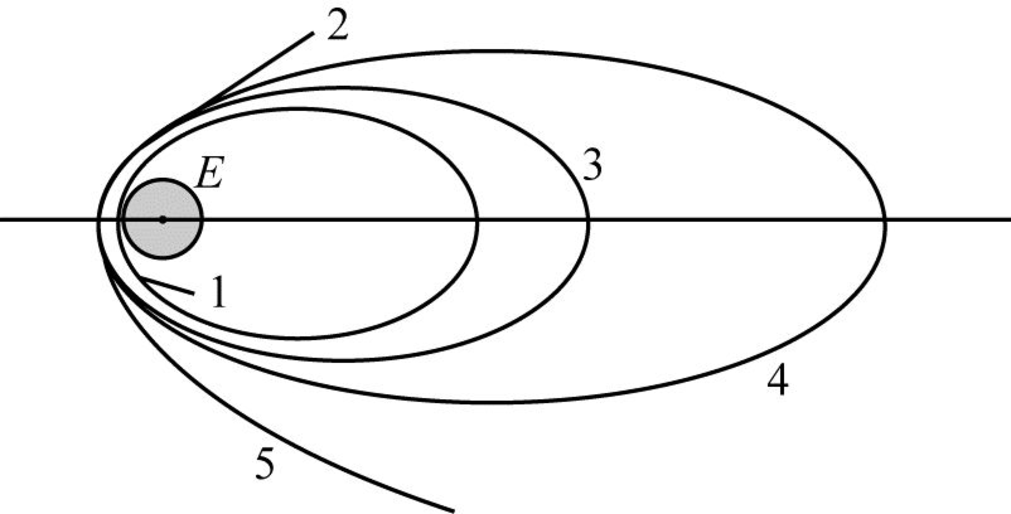
\includegraphics[width = 0.3\textwidth]{images/problem-1.pdf} 
\end{flushright}
\tagged{student}{\vspace*{6cm}}
\begin{taggedblock}{teacher}
解析:
\end{taggedblock}
\end{example}


\begin{example}
	足球射到球门横梁上时,因速度方向不同、射在横梁上的位置有别,其落地点也是不同的。已知球门的横梁为圆柱形,设足球以水平方向的速度沿垂直于横梁的方向射到横梁上,球与横梁间的滑动摩擦系数$\mu=0.70$,球与横梁碰撞时的恢复系数$e=0.70$。试问足球应射在横梁上什么位置才能使球心落在球门线内(含球门上)?足球射在横梁上的位置用球与横梁的撞击点到横梁轴线的垂线与水平方向(垂直于横梁的轴线)的夹角$\theta$(小于$90^0$ )来表示。不计空气及重力的影响。
\tagged{student}{\vspace*{6cm}}
\begin{taggedblock}{teacher}
解析:
\end{taggedblock}
\end{example}

\begin{example}
	图示为低温工程中常用的一种气体、蒸气压联合温度计的原理示意图,M为指针压力表,以 表示其中可以容纳气体的容积;B为测温饱,处在待测温度的环境中,以$V_B$ 表示其体积;E为贮气容器,以$V_E$表示其体积;F为阀门。M、E、B由体积可忽略的毛细血管连接。在M、E、B均处在室温 时充以压强$p_0=5.2*10^5Pa$的氢气。假设氢的饱和蒸气仍遵从理想气体状态方程。现考察以下各问题:
	
	1.关闭阀门F,使E与温度计的其他部分隔断,于是M、B构成一简易的气体温度计,用它可测量25K以上的温度,这时B中的氢气始终处在气态,M处在室温中。试导出B处的温度T和压力表显示的压强p的关系。除题中给出的室温 时B中氢气的压强 外,理论上至少还需要测量几个已知温度下的压强才能定量确定T与p之间的关系?
	
	2.开启阀门F,使M、E、B连通,构成一用于测量20~25K温度区间的低温的蒸气压温度计,此时压力表M测出的是液态氢的饱和蒸气压。由于饱和蒸气压与温度有灵敏的依赖关系,知道了氢的饱和蒸气压与温度的关系,通过测量氢的饱和蒸气压,就可相当准确地确定这一温区的温度。在设计温度计时,要保证当B处于温度低于$T_v=25K$ 时,B中一定要有液态氢存在,而当温度高于$T_v=25K$时,B中无液态氢。到达到这一目的, $V_M+V_E$与$V_B$间应满足怎样的关系?已知$T_v=25K$时,液态氢的饱和蒸气压$p_v=3.3*10^5Pa$ 。
	
	3.已知室温下压强$p_1=1.04*10^5Pa$ 的氢气体积是同质量的液态氢体积的800倍,试论证蒸气压温度计中的液态气不会溢出测温泡B。
\begin{flushright}
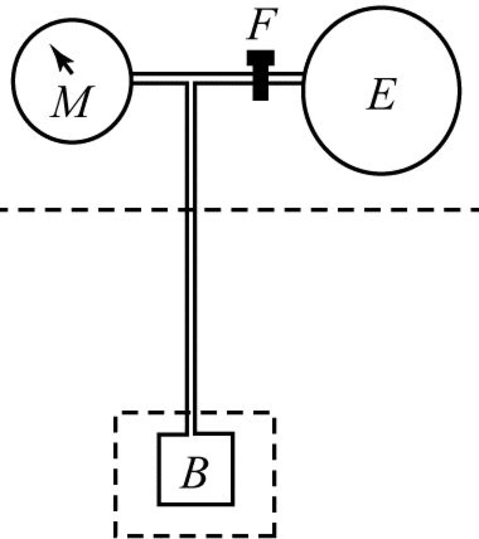
\includegraphics[width = 0.3\textwidth]{images/problem-2.pdf} 
\end{flushright}
\tagged{student}{\vspace*{6cm}}
\begin{taggedblock}{teacher}
解析:
\end{taggedblock}
\end{example}


\begin{example}
	一很长、很细的圆柱形的电子束由速度为v的匀速运动的低速电子组成,电子在电子束中均匀分布,沿电子束轴线每单位长度包含n个电子,每个电子的电荷量为$-e(e>0)$,质量为m。该电子束从远处沿垂直于平行板电容器极板的方向射向电容器,其前端(即图中的右端)于$t=0$时刻刚好到达电容器的左极板。电容器的两个极板上各开一个小孔,使电子束可以不受阻碍地穿过电容器。两极板A、B之间加上了如图所示的周期性变化的电压 $V_{AB}$($V_{AB}=V_A-V_B$,图中只画出了一个周期的图线),电压的最大值和最小值分别为$V_0$和$-V_0$ ,周期为T。若以$\tau$ 表示每个周期中电压处于最大值的时间间隔,则电压处于最小值的时间间隔为$T-\tau$。已知$\tau$的值恰好使在$V_AB$变化的第一个周期内通过电容器到达电容器右边的所有的电子,能在某一时刻$t_b$形成均匀分布的一段电子束。设电容器两极板间的距离很小,电子穿过电容器所需要的时间可以忽略,且$mv^2=6eV_0$,不计电子之间的相互作用及重力作用。
 
	1.满足题给条件的$\tau$和$t_b$的值分别为多少?
	
	2.试在下图中画出$t=2T$那一时刻,在$0-2T$时间内通过电容器的电子在电容器右侧空间形成的电流I,随离开右极板距离x的变化图线,并在图上标出图线特征点的纵、横坐标(坐标的数字保留到小数点后第二位)。取x正向为电流正方向。图中$x=0$ 处为电容器的右极板B的小孔所在的位置,横坐标的单位$s=\sqrt{\frac{eV_0}{m}}$。
\begin{center}
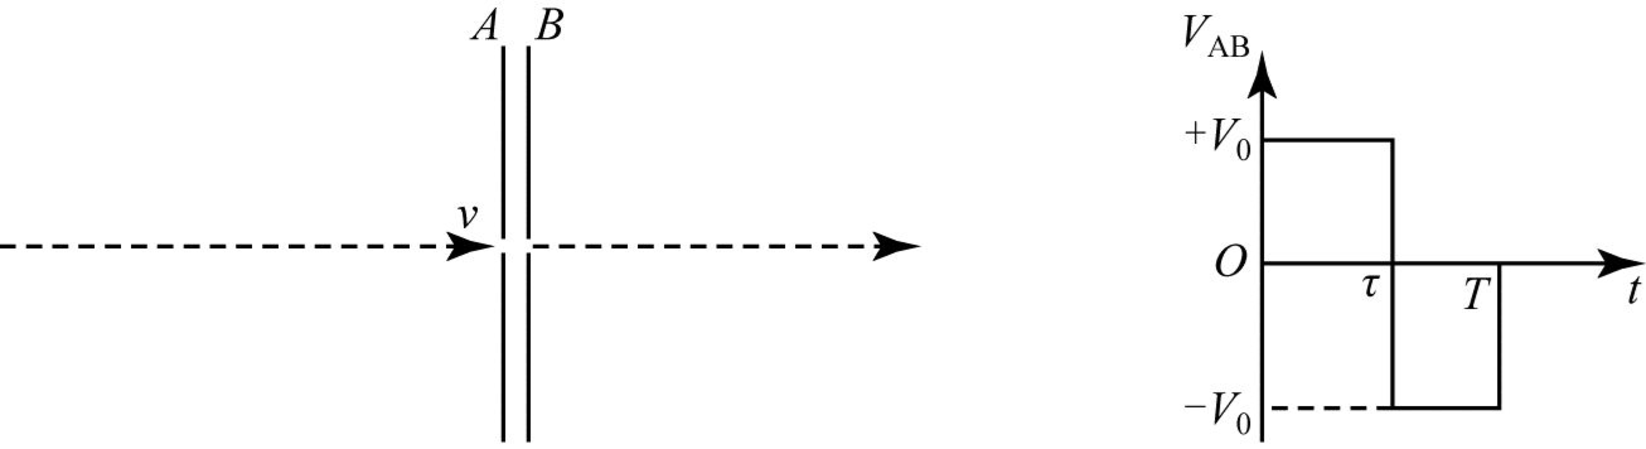
\includegraphics[width = 0.6\textwidth]{images/problem-3.pdf} 
\end{center}
\tagged{student}{\vspace*{6cm}}
\begin{taggedblock}{teacher}
解析:
\end{taggedblock}
\end{example}

\begin{example}
	火箭通过高速喷射燃气产生推力.设温度$T_1$、压强$p_1$的炽热高压气体在燃烧室内源源不断生成,并通过管道由狭窄的喷气口排入气压$p_2$的环境.假设燃气可视为理想气体,其摩尔质量为$\mu$,每摩尔燃气的内能为$u=c_v T$ ($c_v$是常量,T为燃气的绝对温度).在快速流动过程中,对管道内任意处的两个非常靠近的横截面间的气体,可以认为它与周围没有热交换,但其内部则达到平衡状态,且有均匀的压强$p$ 、温度T 和密度$\rho$ ,它们的数值随着流动而不断变化,并满足绝热方程
	\[pV^{\frac{c_v+R}{c_v}}=C\] 
	其中C为恒量,R为普适气体常量,求喷气口处气体的温度与相对火箭的喷射速率.
\tagged{student}{\vspace*{6cm}}
\begin{taggedblock}{teacher}
解析:
\end{taggedblock}
\end{example}

\begin{example}
	两惯性系$S'$与$S$初始时刻完全重合,前者相对后者沿z轴正向以速度v高速运动.作为光源的自由质点静止于$S'$系中,以恒定功率P向四周辐射(各向同性)光子.在S系中观察,辐射偏向于光源前部(即所谓的前灯效应).
	
	1.在S系中观察,$S'$系中向前的那一半辐射将集中于光源前部以x轴为轴线的圆锥内.求该圆锥的半顶角$\alpha$.已知相对论速度变换关系为
	\[u_x=\frac{u'x+v}{1+\frac{u_xv}{c^2}}\]
	式中$u_x$与$u_x'$分别为$S$与$S'$系中测得的速度x分量,c为光速.
	
	2.求S系中测得的单位时间内光源辐射的全部光子的总动量与总能量.

\tagged{student}{\vspace*{6cm}}
\begin{taggedblock}{teacher}
解析:
\end{taggedblock}
\end{example}

\begin{example}
如图,一质量均匀分布的刚性螺旋环质量为m,半径为R,螺距$H=\pi R$,可绕竖直的对称轴$OO'$,无摩擦地转动,连接螺旋环与转轴的两支撑杆的质量可忽略不计。一质量也为m的小球穿在螺旋环上并可沿螺旋环无摩擦地滑动,首先扶住小球使其静止于螺旋环上的某一点A,这时螺旋环也处于静止状态。然后放开小球,让小球沿螺旋环下滑,螺旋环便绕转轴$OO'$转动。求当小球下滑到离其初始位置沿竖直方向的距离为h时,螺旋环转动的角速度和小球对螺旋环作用力的大小。
\begin{flushright}
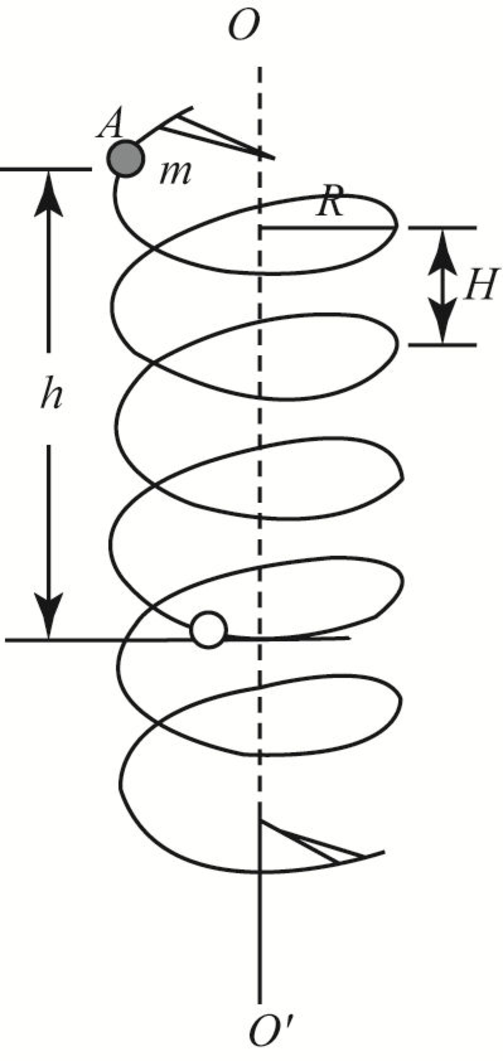
\includegraphics[width = 0.2\textwidth]{images/problem-4.pdf} 
\end{flushright}
\tagged{student}{\vspace*{6cm}}
\begin{taggedblock}{teacher}
解析:
\end{taggedblock}
\end{example}

\begin{example}
如图所示,一质量为m、电荷量为q(q>0)的粒子作角速度为$\omega$、半径为R的匀速圆周运动。一长直细导线位于圆周所在的平面内,离圆心的距离为d(d>R),在导线上通有随时间变化的电流I,$t=0$时刻,粒子速度的方向与导线平行,离导线的距离为d+R 。若粒子做圆周运动的向心力等于电流i的磁场对粒子的作用力,试求出电流i随时间的变化规律。不考虑变化的磁场产生的感生电场及重力的影响。长直导线电流产生的磁感应强度表示式中的比例系数k已知。
\begin{flushright}
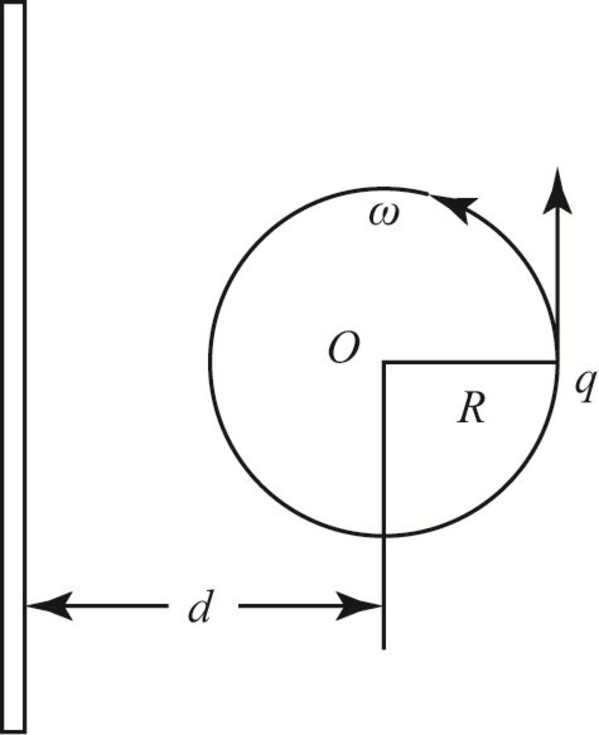
\includegraphics[width = 0.2\textwidth]{images/problem-5.pdf} 
\end{flushright}
\tagged{student}{\vspace*{6cm}}
\begin{taggedblock}{teacher}
解析:
\end{taggedblock}
\end{example}

\begin{example}
如图所示,两个固定的均匀带电球面,所带电荷量分别为$+Q$和$-Q$($Q>0$),半径分别为R和$\frac{R}{2}$,小球面与大球面内切于C点,两球面球心$O$和$O'$的连线MN沿竖直方在MN与两球面的交点B、0和C处各开有足够小的孔因小孔损失的电荷量忽略不计,有一质量为m,带电荷为$q(q>0)$的质点自MN线上离B点距离为R的A点竖直上抛。设静电力常量为k,重力加度为g 。

1.要使质点从A点上抛后能够到达B点,所需的最小初动能为多少?

2.要使质点从A点上抛后能够到达O点,在不同条件下所需的最小初动能各为多少?

\begin{flushright}
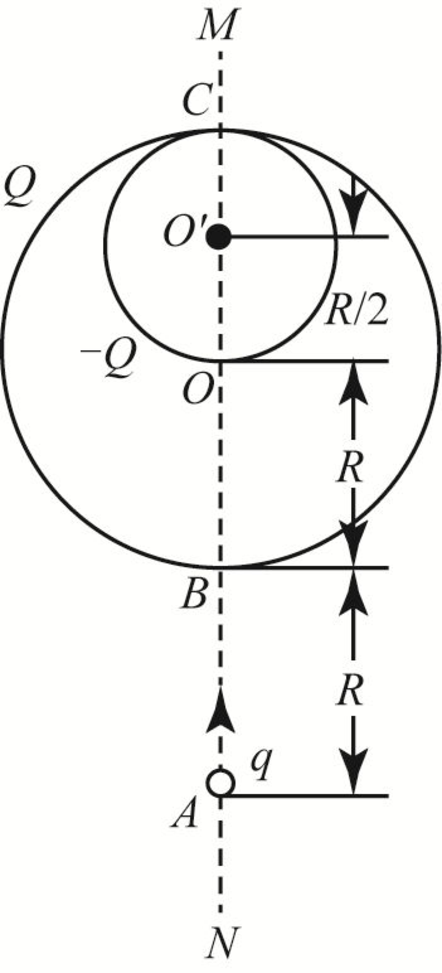
\includegraphics[width = 0.2\textwidth]{images/problem-6.pdf} 
\end{flushright}

\tagged{student}{\vspace*{6cm}}
\begin{taggedblock}{teacher}
解析:
\end{taggedblock}
\end{example}



\begin{example}
	印度物理学家 Chandrasekhar 在1930年提出关于白矮星质量上限的著名理论。
	以下几个问题可以帮助我们理论Chandrasekhar质量极限的概念。
	
	(1)考虑一个质量为$M$,半径为$R$均匀分布的球体,求它的引力势能$E_G$。
	
	(2)假设该恒星完全由氢构成,所有的氢以等离子态存在。
	如果内部核反应已经完全停止,所以没有能量产生,恒星在引力作用将收缩。
	由于Pauli不相容原理,电子不可能处于相同的量子状态,这会导致一个宏观的排斥效果。
	从量子统计学可知这时电子的总能量可以写为
	\[
	E_e = \frac{\hbar^2\pi^3}{10m_e4^{2/3}}\left(\frac{3}{\pi}\right)^{7/3}\frac{N_e^{5/3}}{R^2},
	\]
	其中$N_e$为总电子数。
	给出平衡时白矮星半径和质量的关系。
	对于一颗质量与太阳相同的白矮星,定量计算出它的半径。
	
	(3)估计这颗白矮星内部电子之间的平均距离和速度。
	如果你得到的速度与光速接近,说明其内部的电子实际上是相对论性的,这时正确的电子能量需要用
	\[
	E_e^{rel} = \frac{\pi^2}{4^{4/3}}\left(\frac{3}{\pi}\right)^{5/3}\frac{\hbar c}{R}N_e^{4/3}
	\]
	来代替。重新计算平衡时半径和质量的关系,你发现和非相对论的计算有何不同?
	能否存在一个质量$M_c$使白矮星处于平衡状态。
	
	(4)如果实际白矮星的质量大于$M_c$,那么它将收缩还是膨胀?
	从中你能够得到什么结论?
	
	
	\tagged{student}{\vspace*{4cm}}
	\begin{taggedblock}{teacher}
		
		解析:
	\end{taggedblock}
\end{example}


\begin{example}
由单位长度电阻为r的导线组成如图所示的正方形网络系列.n=1时,正方形网络边长为L,n=2时,小正方形网络的边长为$\frac{L}{3}$;n=3时,最小正方形网络的边长为$\frac{L}{9}$。当n=1、2、3 时,各网络上A、B两点间的电阻分别为多少?
\begin{center}
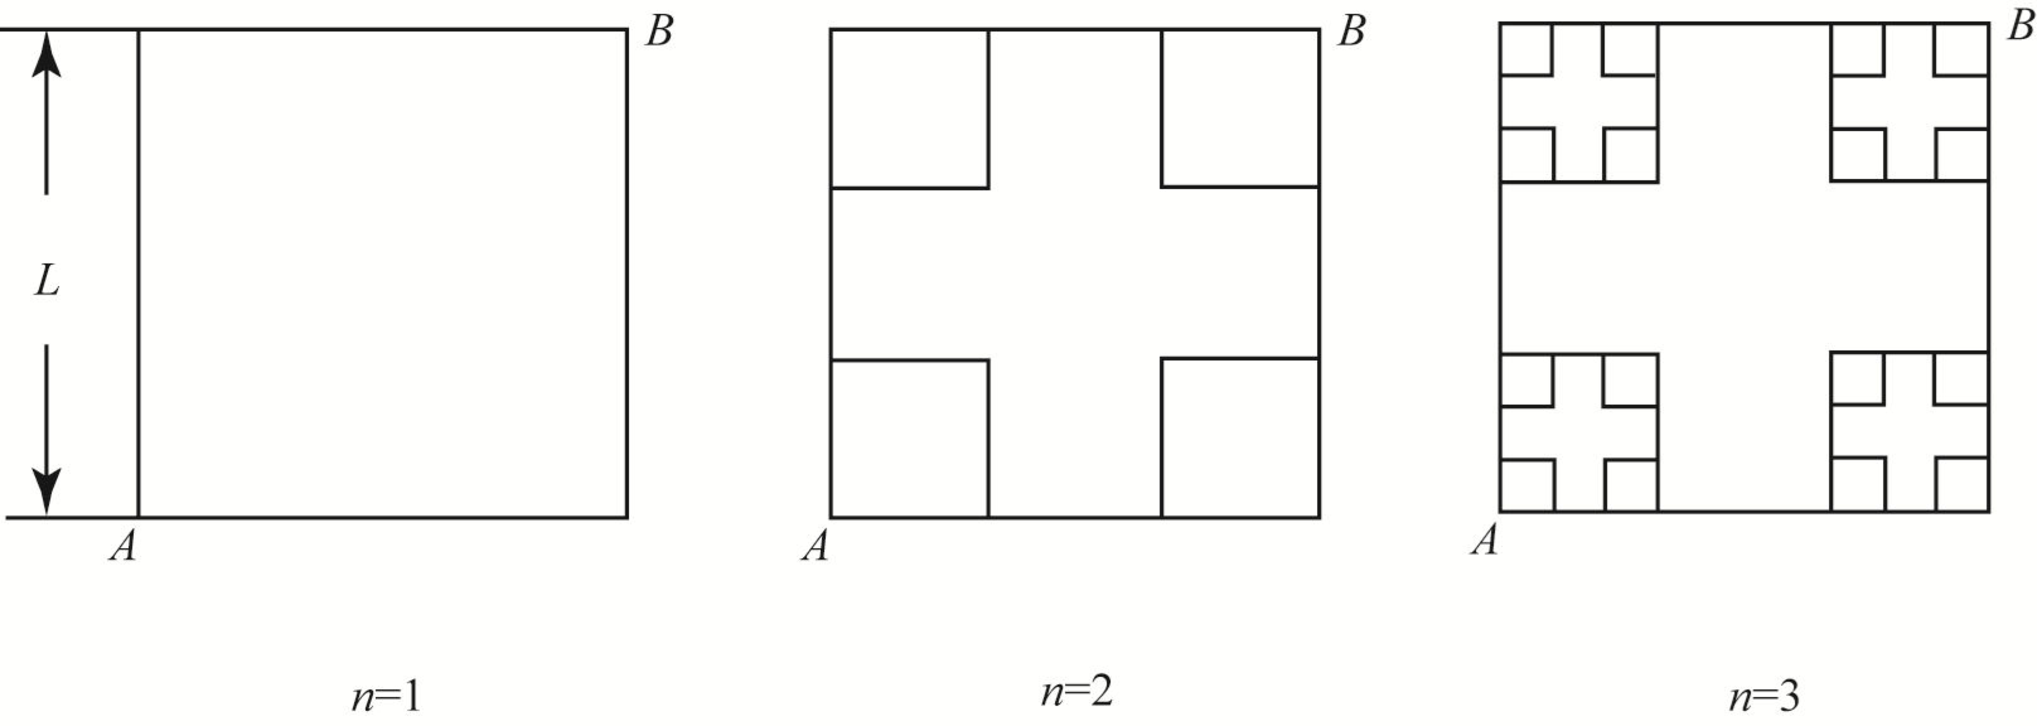
\includegraphics[width = 0.8\textwidth]{images/problem-7.pdf} 
\end{center}
\tagged{student}{\vspace*{6cm}}
\begin{taggedblock}{teacher}
解析:
\end{taggedblock}
\end{example}


\begin{example}
正午时太阳的入射光与水平面的夹角$\theta=45^0$。有一座房子朝南的墙上有一个直径 的圆窗,窗口中心距地面的高度为H。试设计一套采光装置,使得正午时刻太阳光能进人窗口,并要求进入的光为充满窗口、垂直墙面、且光强是进人采光装置前2倍的平行光.可供选用的光学器件如下:一个平面镜,两个凸透镜,两个凹透镜;平面镜的反射率为$80\%$,透镜的透射率为$70\%$ ,忽略透镜表面对光的反射。要求从这些器件中选用最少的器件组成采光装置。试画出你所设计的采光装置中所选器件的位置及该装置的光路图,并求出所选器件的最小尺寸和透镜焦距应满足的条件。
\begin{flushright}
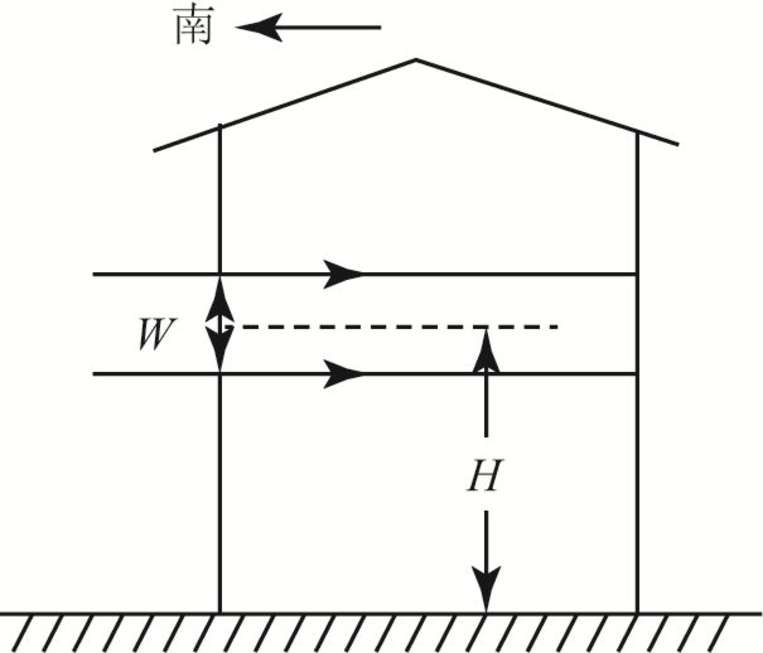
\includegraphics[width = 0.3\textwidth]{images/problem-8.pdf} 
\end{flushright}
\tagged{student}{\vspace*{6cm}}
\begin{taggedblock}{teacher}
解析:
\end{taggedblock}
\end{example}


\begin{example}
已知粒子1 和粒子 2 的静止质量都是$m_0$ ,粒子1静止,粒子2以速度$v_0$与粒子 1 发生弹性碰撞。

1.若碰撞是斜碰,考虑相对论效.试论证:碰后两粒子速度方向的夹角是锐角、直角还是钝角。若不考虑相对论效应结果又如何?

2.若碰撞是正碰,考虑相对论效应,试求碰后两粒子的速度。

\tagged{student}{\vspace*{6cm}}
\begin{taggedblock}{teacher}
解析:
\end{taggedblock}
\end{example}


%%%
%%%%%%%%%%%%%%$$